\documentclass{article}

% if you need to pass options to natbib, use, e.g.:
% \PassOptionsToPackage{numbers, compress}{natbib}
% before loading nips_2018

% ready for submission

\usepackage[]{biblatex}
\addbibresource{bib.bib}

\usepackage[nonatbib]{nips_2018}


% to compile a preprint version, e.g., for submission to arXiv, add
% add the [preprint] option:
% \usepackage[preprint]{nips_2018}

% to compile a camera-ready version, add the [final] option, e.g.:
% \usepackage[final]{nips_2018}

% to avoid loading the natbib package, add option nonatbib:
% \usepackage[nonatbib]{nips_2018}

\usepackage[utf8]{inputenc} % allow utf-8 input
\usepackage[T1]{fontenc}    % use 8-bit T1 fonts
\usepackage{hyperref}       % hyperlinks
\usepackage{url}            % simple URL typesetting
\usepackage{booktabs}       % professional-quality tables
\usepackage{amsfonts}       % blackboard math symbols
\usepackage{nicefrac}       % compact symbols for 1/2, etc.
\usepackage{microtype}      % microtypography
\usepackage[svgnames]{xcolor}

\providecommand\comment[1]{\textbf{COMMENT:} \textcolor{Magenta}{#1}}

\title{Precision from Retrying: Closed-Loop Robotic Manipulation using Self-Supervised Learning}
%%SL.04.20: Let's think about the title a bit more. This seems like a reasonable starting point. But first let's list the main ideas that seem to make the work exciting:
%The ability to fix mistakes
%The ability to reach goal images by comparing them directly to the current image
%The ability to achieve goals to high accuracy
%The ability to do on-policy data collection to acquire more complex skills like grasping
% Some things are exciting, but not inherently new to this work, including: self-supervised, closed-loop, etc.
%  on the other hand, instead of the somewhat generic 'self-supervised learning,' we can probably come up with something
%  a bit more descriptive: one thing that makes our approach different is that, with on-policy data collection, the robot
%  is essentially setting its own goals and then attempting to reach them, so we can call it something like 'self-directed play'
% Some things are exciting but not mentioned, including the fact that this is done with raw images...
% Here are a few thoughts I have about possible titles:
%Visual Learning with Self-Directed Play: Acquisition of Complex Robotic Skills with Direct Video Prediction
%Self-Directed Play with Visual Recall: Learning Manipulation Tasks by Reaching Previous Observations
%Learning Vision-Based Robotic Skills with Self-Directed Play
%...
% Another direction we could go is to emphasize that the method can succeed even with an imperfect predictor, by trying again, but I'm not really sure how to fit that into a very concise title
%%SL.04.20: it would also be good to get some illustrated diagram put together soon to explain how the method works... I feel like a diagram might be quite important here

% The \author macro works with any number of authors. There are two
% commands used to separate the names and addresses of multiple
% authors: \And and \AND.
%
% Using \And between authors leaves it to LaTeX to determine where to
% break the lines. Using \AND forces a line break at that point. So,
% if LaTeX puts 3 of 4 authors names on the first line, and the last
% on the second line, try using \AND instead of \And before the third
% author name.

\author{
  David S.~Hippocampus\thanks{Use footnote for providing further
    information about author (webpage, alternative
    address)---\emph{not} for acknowledging funding agencies.} \\
  Department of Computer Science\\
  Cranberry-Lemon University\\
  Pittsburgh, PA 15213 \\
  \texttt{hippo@cs.cranberry-lemon.edu} \\
  %% examples of more authors
  %% \And
  %% Coauthor \\
  %% Affiliation \\
  %% Address \\
  %% \texttt{email} \\
  %% \AND
  %% Coauthor \\
  %% Affiliation \\
  %% Address \\
  %% \texttt{email} \\
  %% \And
  %% Coauthor \\
  %% Affiliation \\
  %% Address \\
  %% \texttt{email} \\
  %% \And
  %% Coauthor \\
  %% Affiliation \\
  %% Address \\
  %% \texttt{email} \\
}

\begin{document}
% \nipsfinalcopy is no longer used

\maketitle

\begin{abstract}
Self-supervised learning methods, in particular video-prediction has recently been successfully used in robotic manipulation showing that generalizable skills can arise without the need for any external supervision.
%%SL.04.20: It would be a good idea to start with one sentence of fairly broad motivation to explain the bigger context of why the problem matters. It doesn't really need to be specific to video prediction, but more of a broad motivation for self-supervised visual learning of skills.
Self-supervised methods have the advantage that data is collected automatically in large amounts while removing the need for expensive data labeling. However the manipulation skills obtained in this way thus far have been coarse.
%%SL.04.20: not obvious what coarse means
The first contribution of this work is a video-prediction based model-predictive control (MPC)
%%SL.04.20: I'm inclined to suggest leaving the jargon (like MPC) out of the abstract for now, and using more accessible phrasing.
algorithm that achieves high precision by incorporating a learned image-to-image registration module that allows a user to specify target states precisely using goal-images. The model-predictive control algorithm continuously registers the current observations to the goal image allowing it to correct for prediction errors by "retrying" until the goal is achieved. 

Past self-supervised learning approaches collect data by applying random actions thus restricting range of states where the learned model is valid. The second contribution is a method for directing the data collection towards task-relevant areas of the state space. We propose a method that leverages small numbers of demonstrations and collects additional on-policy data by running the proposed model-predictive control algorithm with an automatically selected goal. In addition to using demonstrations our method also allows for making use of prior domain knowledge to further improve the data collection process: Data collection can be started with simple hand-engineered policies that only requires a very low success rates.
\end{abstract}
%%SL.04.20: Here is my attempt at an alternative abstract that I thing brings out some of the more exciting things about the work. Maybe this can serve as some inspiration for how to get a more focused abstract in place that at the same time still touches on the big picture stuff:
%Understanding how the world works -- which actions lead to which future events -- can allow humans and animals to act intelligently in complex and unfamiliar situations. Crucially, understanding and predicting physical interactions does not require any supervision beyond observation of one's own actions and their consequences. This makes prediction an appealing objective for self-supervised learning of behavioral skills, for example for autonomous robots. However, incorporating prediction of future sensory inputs into an end-to-end framework for decision making and control poses a number of major challenges. How should the data for learning to predict be collected? How should the predictive model be used? What happens when the predictions are inaccurate? In this paper, we tackle these questions by proposing a method for learning complex robotic skills from raw image observations, using only autonomously collected experience. Our method is based on two key ideas. First, we use self-directed play to collect data, where the robot autonomously proposes goals and then attempts to execute them. We demonstrate in simulation that this substantially improves performance over random data collection. Second, we observe that even an imperfect model can complete complex tasks if it can continuously retry, but this requires the model to not lose track of the objective (e.g., the object of interest). By incorporating end-to-end learned registration into our method, we can enable the robot to continuously retry the task until it gets it right. We demonstrate that these two ideas can be combined to enable complex behaviors to be learned from scratch using only raw visual inputs, including grasping and repositioning objects, non-prehensile pushing, and maneuvering objects around obstacles. Our real-world experiments demonstrate a model trained with ??? hours of autonomously collected experience with self-directed play, and testing on previously unseen objects.

\section{Introduction}

\begin{wrapfigure}{r}{.4\columnwidth}
\vspace{-5mm}
\centering
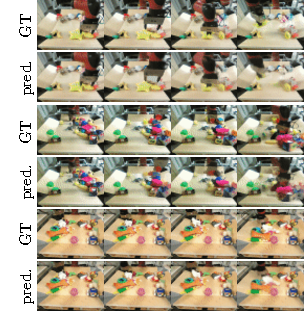
\includegraphics[width=0.4\columnwidth,trim={3.2mm 0 0 0},clip]{images/video_prediction}
\caption{\small{Ground truth and predictions from the model (only every 4 frames are shown). These examples show grasping, pushing, and simultaneous grasping and dragging. \todo{consider replacing with sudeep diagram?}}}
\label{fig:video_prediction}
\vspace{-0.2in}
\end{wrapfigure}

Humans have the ability to learn complex skills such as manipulating objects through millions of interactions with their environment during their lifetime.
These interactions enable us to acquire a general understanding of the physical world and, notably, do not require significant supervision beyond observation of one's own actions and their consequences. Hence, self-supervised learning through prediction is an appealing direction of research as it enables intelligent systems to leverage and learn from massive amounts of unlabeled raw data to autonomously acquire general skills. Yet, self-supervised learning systems using predictive models of sensory inputs present a number of challenges: planning needs to account for imperfections in the predictive model and the robot needs a grounded mechanism for evaluating predicted futures.
How can we enable systems to plan to perform complex tasks from raw sensory observations, even when the predictions are not always accurate?

Prior work on self-supervised robot learning has enabled robots to learn rudimentary, short-term manipulation skills such as grasping~\cite{lerrel,google_handeye}, singulation~\cite{princeton_pushgrasp}, pushing~\cite{foresight,sna}, poking~\cite{pulkit}, and other arm motions~\cite{se3_control}. The question that we are concerned with in this work is: can self-supervised predictive models of raw visual observations be used to perform more complex and realistic tasks, especially tasks that are temporally extended? 
%, closed-loop control of multiple forms of behavior and goals through self-supervision remains an open problem.
%Prior work has demonstrated that video prediction can be used for rudimentary, short-term robotic manipulation tasks in the real world, such as pushing objects~\cite{}. The question we are concerned with in this work is: can direct video prediction be used to perform more complex and realistic tasks, especially tasks that are temporally extended? 
While this might seem exceedingly challenging due to the difficulty of long-term prediction of images, we make use of the well-known principle of model-predictive control (MPC) that allows targeting long-terms goals with a relatively short prediction horizons. To allow effective replanning, we need a planning objective that allows the robot to reliably make progress towards the goal.
%that is optimized by a short-horizon planner allowing to reliably make progress towards the goal. 

%While this might seem exceedingly challenging due to the difficulty of long-term prediction of images, we make the following observation: that make it feasible to perform relatively long-horizon tasks. First, we observe that short-horizon planning can still give us a good indication of the potential for a plan to achieve a long-term goal, if provided with the right cost function. This fact has been known for decades, and is the basis for model-predictive control: iterative short-horizon replanning that aims to achieve long-term goals. Yet, maintaining an accurate estimate of the cost function throughout planning is crucial.
We propose a cost function based on image-to-image registration, which we demonstrate can itself be learned without any human supervision using the same exact dataset as the one used to train the predictive model. The key element that enables our method to perform long-horizon tasks is that, using our cost function, the robot can always evaluate the distance to the goal, allowing it to continuously retry, so that even flawed predictions allow for an eventual successful execution. 



%Closed-loop control allows the robot to be persistent, correcting for mistakes caused by inevitable model inaccuracies and continuously retrying until it succeeds.
%Further, learning models that can be used to plan multiple types of behaviors is critical for learning general-purpose control.
%%SL.06.12: there are two ideas above: (1) learning models that can be used for various tasks is important for general-purpose control (2) retrying is a good idea; these ideas are kind of stuck together awkwardly a bit, can we push them apart so that one builds on the other?
%In this work, we aim to develop a learning system that interacts with the environment autonomously, building a model that can be used to plan a variety of motions, including pushing, grasping, and placing, while enabling the agent to continuously try and retry the task until it succeeds.
%%SL.06.12: the title says something about being precise -- where does that come in?

%A robot equipped with action-conditioned predictive models of future observations has some understanding of the physical world and how it changes as a consequence of its actions. Such model could then be used by the robot to plan multiple types of behaviors for general-purpose control. These models can be learned through self-supervision, whereby the robot interacts with the environment through random actions while observing through its sensors. In our work, we use a video prediction model that predicts future frames conditioned on actions and past frames.

%%AL.06.13: I think we need two paragraphs that contains the following information:
% Paragraph on self-supervised learning. Massive amounts of self-supervised data. Action-conditioned video prediction model that predicts future frames by implicitly transforming pixels from previous frames via image-space flow fields. These flows can be used for planning given a designated pixel position in the first frame and goal pixel position in the goal frame (say how it's done). Forward models can deviate from the truth very quickly due to compounding errors. Naturally, replanning (MPC). However, we don't have good cost functions since we have lost designed pixel position in the new first frame. Solution?
% Paragraph on registration. Track designed pixel position. Allows for more precise retrying. Registration registers to both first and goal frames, so can be accurate near beginning and end of trajectory.


%%SL.04.20: I would recommend reading through this carefully and noting the key points that we need to touch on in an introduction: https://cs.stanford.edu/people/widom/paper-writing.html


We demonstrate our method on the task of maneuvering unknown objects in a table-top setting using a robot manipulator. To autonomously learn to perform manipulation skills with high-fidelity, tasks need to be specified in way that allows for precision and retrying. We specify a goal by providing an image of the desired configuration along with user-annotated positions of the objects of interest\footnote{This also allows the user to specify distractor objects that can be ignored in the goal image}. This provides a straight-forward and grounded mechanism for a human to provide a goal in the observation space of the robot.
Building upon prior methods that use self-supervised predictive models for control~\cite{foresight,sna,se3_control}, we develop a method that can plan actions with a video prediction model to achieve the desired state specified in the goal image.
%%SL.06.12: I feel like maybe we should explicitly say that our method builds on prior work (foresight, sna), since in this case the contribution might actually be easier to understand if we explicitly frame it in terms of prior work. It might open us up to accusations that the work is incremental, but I think that is less bad than a lack of clarity about the nature of the contribution

The main contribution of this work is a method for computing the planning cost based on image-to-image registration by using a learned registration model to find correspondences  between the current image and both the goal image and the initial image.
%We train a deep convolutional network to find these correspondences by learning an image-to-image warping function in a self-supervised manner. 
This allows closed-loop control, enabling the robot to persistently attempt the task until completion. In contrast to the short-horizon pushing skills and arm motions demonstrated in prior work~\cite{foresight,sna,se3_control}, we show that our video prediction model can be used to perform longer-term manipulations, autonomously choosing when to push or to  pick objects, and, when provided enough time, accomplish tasks significantly more consistently.
In addition we show that a joint pushing and grasping-policy can be emerge from pure self-supervised learning. Furthermore by using with two separate views for video-prediction and task specification, 3D-tasks manipulation tasks can be solved.

%Compared to prior work on self-supervised learning and hand-engineered tracking modules, we find that our approach is able to perform a variety of object manipulation tasks and, when provided enough time, achieve tasks significantly more consistently.

%%SL.06.12: Some high level comments on the introduction: Currently, it doesn't really talk about grasping -- it just abstractly says that there are multiple skills, but not what those skills are. Can we elaborate on this point a little bit? I think the current intro is definitely better, but we should try to do a better job of coming up with the story. I think we should make sure we touch on the following points/questions:
%Prior work has demonstrated that video prediction can be used for rudimentary, short-term robotic manipulation tasks in the real world, such as pushing objects~\cite{}. The question we are concerned with in this work is: can direct video prediction be used to perform more complex and realistic tasks, especially tasks that are temporally extended? While this might seem exceedingly challenging due to the difficulty of long-term prediction of images, we make the following observations that make it feasible to perform relatively long-horizon tasks. First, we observe that short-horizon planning can still give us a good indication of the potential for a plan to achieve a long-term goal, if provided with the right cost function. This fact has been known for decades, and is the basis for model-predictive control: iterative short-horizon replanning that aims to achieve long-term goals. For video prediction, we propose a cost function based on image registration, which we demonstrate can itself be learned without any human supervision using the same exact dataset as the one used to train the predictive model. The second idea that enables our method to perform long-horizon tasks is that, if the robot can always evaluate the goal, it can continuously retry, so that even flawed predictions allow for an eventual successful execution. We use the same learned registration model to enable this retrying behavior.
%
%In contrast to the short-horizon pushing skills demonstrated in prior work~\cite{}, we show that our video prediction model can be used to perform longer-term manipulations and automatically choose to push and pick objects, acquiring rudimentary grasping behaviors entirely via video prediction.

%this registration network learns a function that transforms images from arbitrary timesteps along a video to match frames from other timesteps. 










\printbibliography
\end{document}
